\section{Aonde Queremos Estar}

Uma vez em que estivermos rodando os nossos trabalhos no ``Estado de arte'', sobrará muito tempo livro para criarmos e inovamos. 

% Por exemplo, imagine se a Hotmart fosse da seguinte maneira:
% % \begin{figure}[H]
% %     \centering
% %     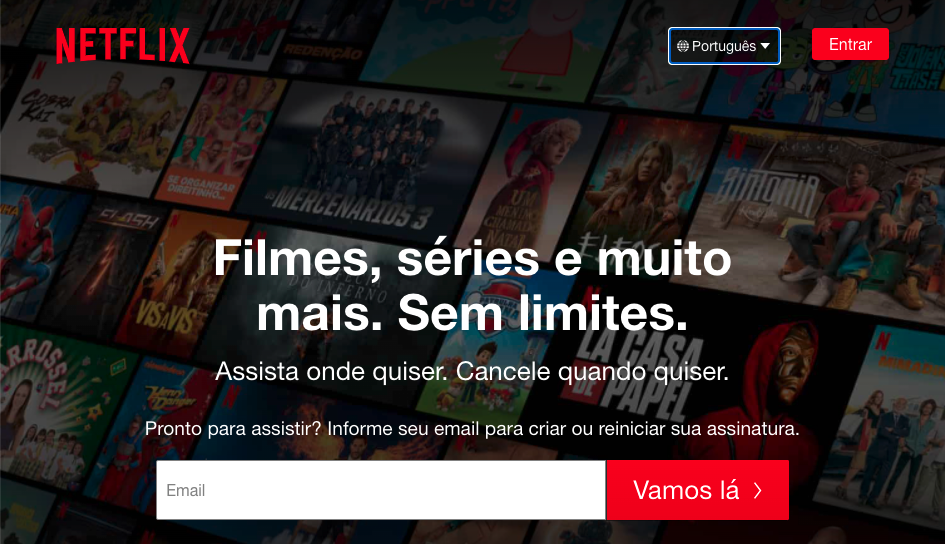
\includegraphics[scale=0.37,keepaspectratio=true]{images/04.png}
% %     \caption{Tela de login independente de haver compras}
% % \end{figure}

% % \begin{figure}[H]
% %     \centering
% %     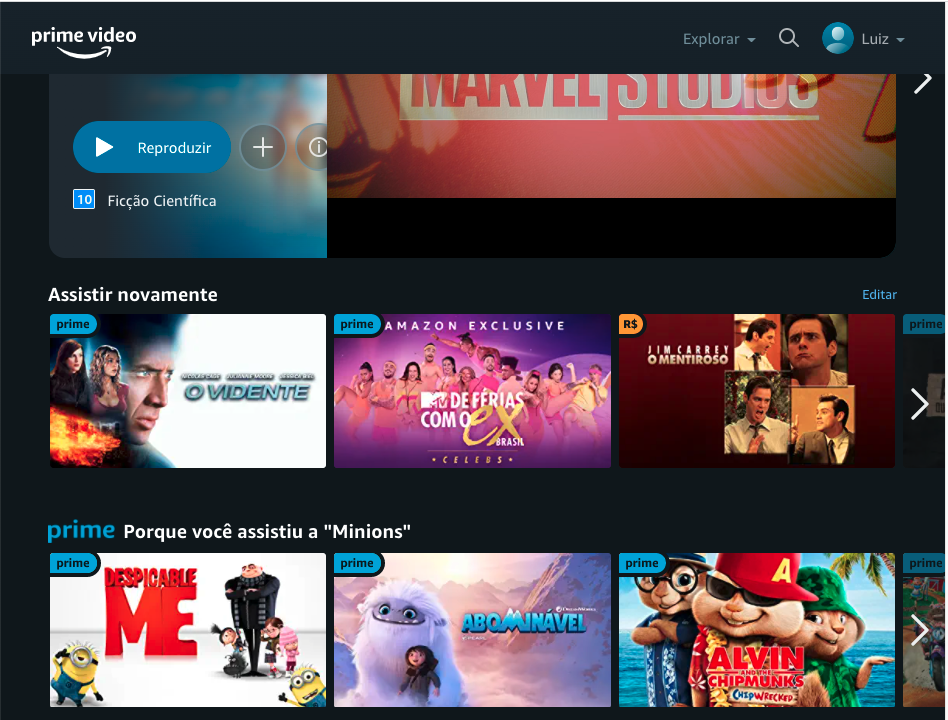
\includegraphics[scale=0.30,keepaspectratio=true]{images/05.png}
% %     \caption{Novidades do catálogo Hotmart, conteúdo gratuito oferecido pelo produtor como um trailer de seu produto}
% % \end{figure}

% % \begin{figure}[H]
% %     \centering
% %     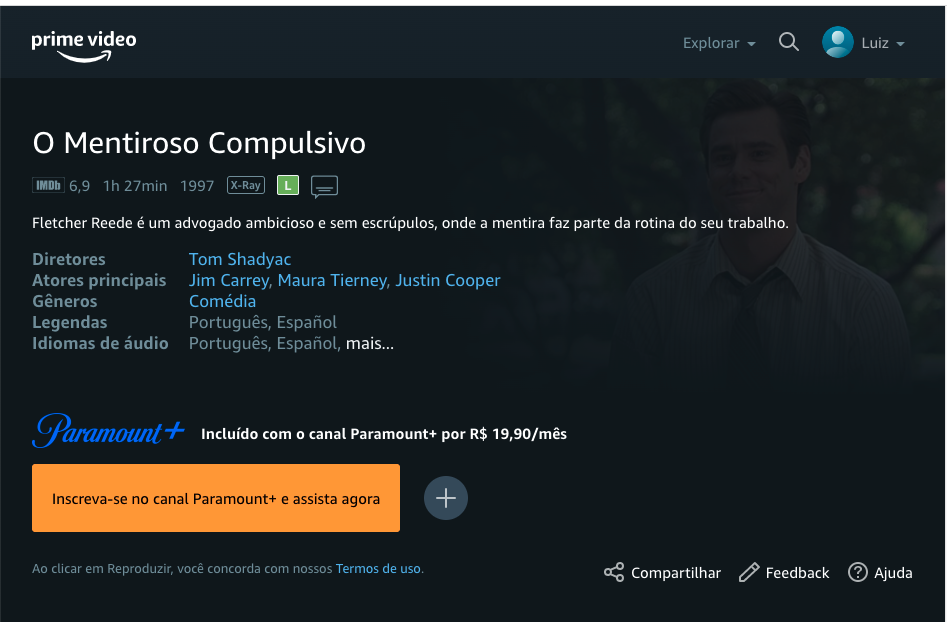
\includegraphics[scale=0.40,keepaspectratio=true]{images/06.png}
% %     \caption{Página de vendas de um pequeno, médio ou grande produtor}
% % \end{figure}

% % \begin{figure}[H]
% %     \centering
% %     
\includegraphics[scale=0.50,keepaspectratio=true]{images/07.png}
% %     \caption{Tela superior deve conter: COMPRAR - MINHAS COMPRAS - VENDER - MINHAS VENDAS - AJUDA}
% % \end{figure}

% \section{Conclusão}

% Acredita-se que se a plataforma por voltada para o comprador, conseguiremos melhores performances justamente pelo efeito orgânico da internet. A ideia é posicionar a Plataforma onde YouTube, Amazon Prime e Netflix não posicionaram. Seria ficar ali no meio deles servindo o que eles não servem. 

% Imagine ver aquela gameplay completinha do seu gamer favorito pagando 3,99 sem anúncio? e ainda ter uma porrada de funcionalidade exclusiva. Seria muito melhor, pelo menos eu acho. E eles têm muitas dores com o YouTube onde sao cancelados por direitos autorais. Na nossa plataforma, ele poderia colocar uma música do Pink Floyd se quisesse desde que recolhesse os direitos aos autores. Seria um modelo onde todo mundo ganha.

% Poderíamos aplicar o reembolso que nem na Steam: jogou por mais de 2 horas, sem reembolso. Isso iria reduzir bastante demanda de suporte e ticket pra gente. 

% Fora que poderíamos fazer parcerias com as universidades para aprimorar nossos algoritmos de classificação, clusterização e sistema de busca e recomendação. 
